%\section{Conditions and Loops}
In many cases, we want to iterate certain processing steps many times (see "Loops" in the figure \ref{fig_scriptscheme}), or we want to limit some of the process in the program only for certain situations (see "Conditions": in the figure \ref{fig_scriptscheme}). In this section we learn how to include these loops and conditional behaviors into macro. 

\begin{figure}[htbp]
\begin{center}
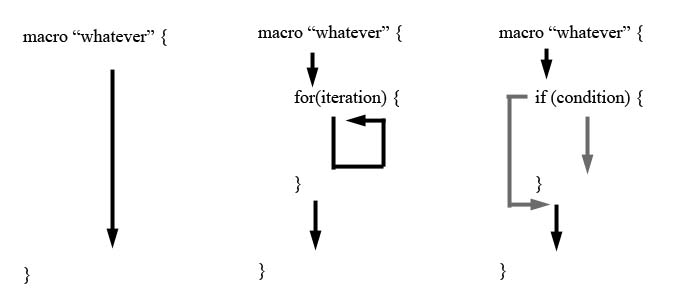
\includegraphics[width=\textwidth]{fig/fig23_1_ScriptSchemes.png}
\caption{Schematic view of conditions and loops. Straightly top to bottom, line by line processing (left) and macro with loops (middle) and with a condition (right).} \label{fig_scriptscheme}
\end{center}
\end{figure}

\subsection{Loop: for-looping}
Here is a simple example macro using for-loop. Write the macro in your editor and run it. 
\lstinputlisting[morekeywords={*, for}]{code/code09.ijm}
The result should look like figure \ref{fig_whateverOut}.

%whatever x 5 figure
\begin{figure}[h!]
\begin{center}
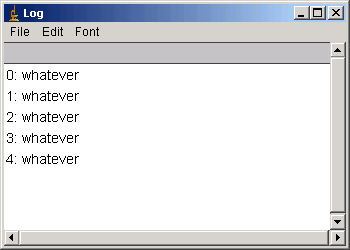
\includegraphics[scale=0.6]{fig/fig2311_whatever5.png}
\caption{Code 9 output in Log Window}
\label{fig_whateverOut}
\end{center}
\end{figure}

\begin{itemize}
\item Line 3 asks the user to input a string (we did this already). 
If user does not change the default text ("whatever") and click "OK", 
then the macro interpreter proceeds to line 4.

\item Line 4 \ilcom{for( i = 0 ; i < 5 ; i+= 1)} sets the number of loops. 
Three parameters are required for "for" loop. The first parameter defines the variable used for the counting loop and its initial value (\ilcom{i = 0}). The second parameter sets the condition for exiting from the loop (\ilcom{i < 5}). Third parameter sets the step size of i, meaning that how much value is added per loop (\ilcom{i += 1}, could also be subtraction, multiplication, division e.g. \ilcom{i -= 1}).
Spaces between variables, numbers, operators and separators (e.g. semicolon, parenthesis) can be ignored and they could be written continuously. Macro runs without those spaces. However, this is not recommended for keeping a better readability of the code. Don't try to rush, make spaces!
\item After this \ilcom{for(\ldots;\ldots;\ldots)} statement, there is a brace (\{) at the end of line 4 and the second one  (\}) in the line 6. These curly braces tell ImageJ to loop macro functions in between so the function in line 5 will be iterated according to the parameters defined in the parenthesis of \ilcom{for}. 
Between braces, you could add as many more lines of macro functions as you want, including inner \ilcom{for}-loops and \ilcom{if-else} conditions.
\end{itemize}
So when the macro interpreter reaches line 4 and sees \ilcom{for(}, it starts looking inside the parenthesis and defines that the counting starts with 0 using a variable \ilcom{i}, and then line 5 is executed. The macro prints out "0 \ensuremath\colon whatever" using the content of \ilcom{i}, string \ilcom{\ensuremath\colon} and the string variable \ilcom{txt}. 
Then in line 6 interpreter sees the boundary \ilcom{\}} and goes back to line 4 and adds 1 to i (because of \ilcom{i+=1}). i = 1 then, so \ilcom{i<5} is true. The interpreter proceeds to line 5 and executes the macro function and prints out "1\ensuremath\colon whatever".  Such looping will continue until i = 5, since only by then \ilcom{i<5} is no longer true so interpreter exits from the for-loop. \\


\begin{indentexercise}{1}
(1) Change the first parameter in \ilcom{for(i=0;i<5;i+=1)} so that the macro prints out only 1 line. 

(2) Change the second parameter in \ilcom{for(i=0;i<5;i+=1)} so that the macro prints out 10 lines. 

(3) Change the third parameter in \ilcom{for(i=0;i<5;i+=1)} so that the macro prints out 10 lines. 
\end{indentexercise}


\subsubsection{Stack Analysis by for-looping}
\label{sec:forloopStack}
One of frequently encountered tasks is image stack management, 
such as measuring dynamics or multi-frame processing. 
Many ImageJ functions work with only single frame within a stack. 
Without macro programming, you need to execute the command while you flip the frame manually. 
Macro programming enables you to automate this process. 
Here is an example of measuring intensity change over time\footnote{What we write as macro here could be done with a single command \ilcom{[Image > Stacks > Plot Z-Profile]} but this only measures intensity. If you want to measure other values such as the minimum intensity, a macro should be written. }. 
\lstinputlisting[morekeywords={*, run, setSlice, nSlices}]{code/code10.ijm}
\begin{itemize}
\item Line 3: \ilcom{nSlices} is a macro function that returns the number of slices in the active stack. 

\item Line 4: Sets measurement parameters, from the menu would be \ilcom{[Analyze > Set measurements\ldots]}. In this case "mean min integrated" is added as part of the second argument. ``mean'' is the mean intensity, ``min'' is the minimum intensity and ``integrated'' is integrated density (total intensity). These keys for measured parameters could be known by using the command recorder. 
You do not have to care for now about the "redirect" argument. ``decimal'' is the number of digits to 
the right of the decimal point in real numbers displayed in the results table. 

\item Line 5: clears the results table. 

\item Line 6 to 9 is the loop. Loop starts from count i=0, and ends at i=frame-1. \ilcom{i++} is another way of writing \ilcom{i = i + 1}, so the increment is 1.  

\item Line 7: calculates the current frame number. 

\item Line 8: \ilcom{setSlice} function sets the frame according to the frame number calculated in line 6. 

\item Line 9:  actual measurement is done. 
Result will be recorded in the memory and will be displayed in the Results table window. 
\end{itemize}

Open an example stack \textbf{1703-2(3s-20s).stk}
\footnote{Some of you may realize that you used this sequence 
in the Image Processing / Analysis Course for learning 
stack measurements using Z-profiler \ilcom{[Image > Stacks > Plot Z-Profile]}. Now, you can program similar 
device in macro. 
Good thing about the custom program
is that you will be able to modify the program further to add more functions.
For example, You could measure the time course of standard deviation of
intensity within the selected ROI.}. This is a short sequence of FRAP analysis,
so the edge of the one of the cells is bleached and then fluorescence signal at that bleached position recovers by time. 
Select the frapped region by ROI tool (such as in the figure below). 
Execute the macro. Results will be printed in the Results window (see the table in the figure right: this table is showing only "Mean" column as only ``Mean Intensity'' was selected in the measurement option). 

\begin{figure}[htbp]
 \centering
% \subfloat[Setting a Segmented ROI at the FRAPped area.]{\label{fig:gull}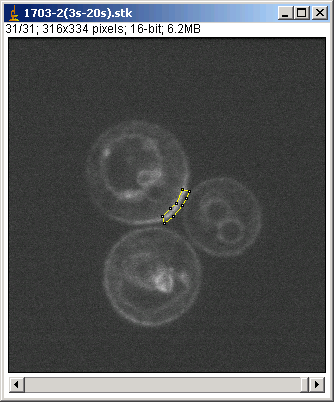
\includegraphics[width=0.3\textwidth]{fig/fig2321a_frapimage.png}}
 \subfloat[]{\label{fig:frapimage}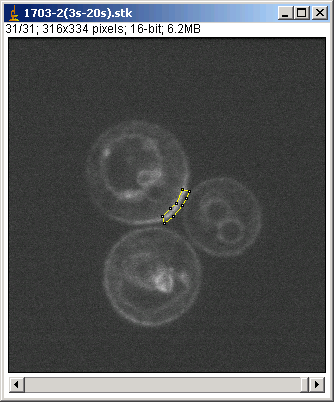
\includegraphics[height = 60mm]{fig/fig2321a_frapimage.png}}
 \quad
 \subfloat[]{\label{fig:frapmeasured}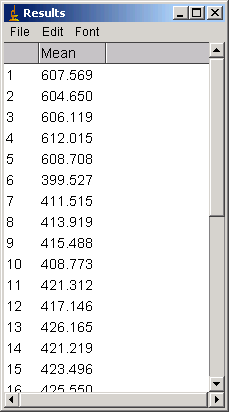
\includegraphics[height = 60mm]{fig/fig2321b_frapResults.png}}
 \caption{Measuring Stack Intensity Series. (a) Setting a Segmented ROI at the FRAPped area. (b) Results of Measuring Mean Intensity Dynamics.}
 \label{fig:frapresults}
\end{figure}


Measurement parameters can be added as argument by modifying the line 4 in the code 10. "Set Measurement" could be added with more parameters to be measured, and the digits after the decimal point could be increased by increasing the number after ``decimal=''. For example, 
\begin{lstlisting}[numbers=none]
run("Set Measurements...", "area mean standard modal min centroid center perimeter bounding integrated median stack redirect=None decimal=5");
\end{lstlisting}

\begin{indentexercise}{1}
Modify code 10 to include more measurement parameters (whatever you like), and test the macro. Check the results. 
\end{indentexercise}

% figure
\begin{figure}[htbp]
\begin{center}
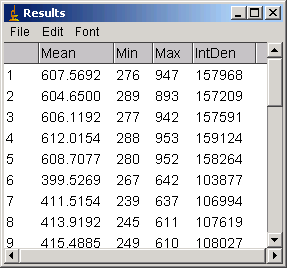
\includegraphics[scale=0.5]{fig/fig2322_moreResultsTable.png}
\caption{An example result after adding more measurement parameters.}
\label{fig_MoreMeasurementPara}
\end{center}
\end{figure} 


\subsection{Loop: while-looping}

Another way of letting a part of macro to loop is \textbf{while}-statement. In this case, iteration is not defined strictly. Looping continues until certain condition is met. As soon as the condition is violated, macro interpreter goes out from the loop.

\subsubsection{Basics of while statement}
Here is a simple example macro using \ilcom{while}.
\lstinputlisting[morekeywords={*, while}]{code/code11.ijm}
This macro prints out characters 0 to 90 with a 10 increment. 

%figure
\begin{figure}[htbp]
\begin{center}
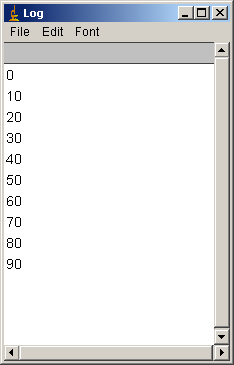
\includegraphics[scale=0.4]{fig/fig2331_Code11out.png}
\caption{Output of code 11}
\label{fig:code11 output}
\end{center}
\end{figure} 

\begin{itemize}
\item line 3: The macro interpreter first assigns 0 to the counter.
\item line 4: The interpreter evaluates if the counter value is less than or equal to 90. Since counter is initially 0\ldots 
\item line 5: Printing function is executed. 
\item line 6: counter is added with 10. 
\item line 7: the interpreter realizes the end of "while" boundary and goes back to line 4. Since counter= 10 <= 90, line 5 is again executed\ldots and so on. When counter becomes 100 in line 6 after several more loops, counter is no longer <=90. So the interpreter goes out from the loop, moves to line 8. Then the macro is terminated.
\end{itemize}

Line 5 could be written in the following way as well.
\begin{lstlisting}[numbers=none]
counter += 10;
\end{lstlisting}
This means that "counter" is added with 10. Similarly, subtracting 10 from counter is 
\begin{lstlisting}[numbers=none]
counter -= 10;
\end{lstlisting}
Multiplication is 
\begin{lstlisting}[numbers=none]
counter *= 10;
\end{lstlisting}
Division is
\begin{lstlisting}[numbers=none]
counter /= 10;
\end{lstlisting}
If the increment is 1 or -1, (counter +=1 or counter-=1), then one could also write them  as 
\begin{lstlisting}[numbers=none]
counter++;
 or 
counter--;
\end{lstlisting}
These two last macro functions are said to work faster than +=1 or -=1, but I myself do not see much difference. Computers are fast enough these days. 

\begin{indentexercise}{1}
(1) Try changing code 11 so that it uses "+=" sign.\\
(2) Change code 11 so that it uses "++" sign, and prints out integers from 0 to 9.\\
\end{indentexercise}
Evaluation of \ilcom{while} condition could also be at the end of loop. In this case, \ilcom{do} should be stated at the beginning of the loop. With do-while combination, the loop is always executed at least once, regardless of the condition defined by \ilcom{while} since macro interpreter reads lines from top to bottom. Try with the following exercise.

\begin{indentexercise}{2}
Change line 4 of code 11 to \ilcom{while (counter <0)} and check the effect (see below).
\end{indentexercise}

\lstinputlisting[morekeywords={*, while}]{code/code11_5.ijm}

Condition for the while-statement could be various. Here is a small list of comparison operators.

\begin{indentCom}
 \begin{tabular*}{0.5\textwidth}{ l r }
< & less than \\
<= & less than or equal\\ 
> & greater than\\ 
>= & greater than or equal to\\
== & equal\\
!= & not equal\\
 \end{tabular*}
\end{indentCom}

\begin{indentexercise}{3}
Modify code 11 so that the macro prints out numbers from 200 to 100, with an increment of -10. 
\end{indentexercise}

\subsubsection{Why is there while-loop?}

An often raised question with the while-loop is why do we have two types of loops, 
the for-loop and the while-loop. Answering to this question, they have different
flexibility. The for-loop is rather solid and the while-loop is more flexible. In the
example code below, the user is asked for a correct number and if the answer is wrong, the
question is asked 5 times repeatedly. Number of loop is not determined by the
programmer, but interactively when the code is running. We will study
the branching of the program based on if-else in the next section.  

\lstinputlisting[morekeywords={*, while}]{code/code11_6.ijm}

Writing a similar code using the for-loop is possible but the code becomes tricky.
Below is the for-loop version of the above code.  

\lstinputlisting[morekeywords={*, for}]{code/code11_7.ijm}

Note that the third argument of for-loop is missing. Since the variable
\ilcom{correct} does not change as long as the answer is wrong, we leave it not
incrementing nor decrementing. In such case we can leave the third argument
vacant. 

\subsection{Conditions: if-else statements}
\subsubsection{Introducing if-else}
A macro program could have parts which are executed depending on some
conditions.
Here is an example of macro with conditions.
\lstinputlisting[morekeywords={*, if}]{code/code12.ijm}
\begin{itemize}
\item Line 3 The macro asks user to input a number and the number is substituted to the variable input\_num.
\item Line 4 Content of input\_num is evaluated. If input\_num is equal to 5, line 5 is executed and prints out the message in the Log window. Otherwise macro interpreter jumps to line 7, and ends the operation.  By adding "else" which will be executed if input\_num is not 5, the macro prints out message in all cases (see code 12.5 for this if - else case). 
\item Line 4 We used double equal signs for evaluating the value in the right side and the left side (e.g. \ilcom{if (a==5)}). 
Note that the role of the sign \ilcom{=} is different from assignments, or substitution (e.g. \ilcom{a = b + c}).
\end{itemize}
%figure
\begin{figure}[htbp]
\begin{center}
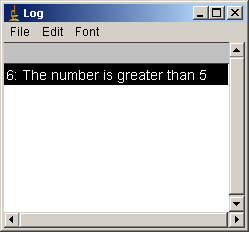
\includegraphics[scale=0.6]{fig/fig2341_code12out.png}
\caption{Output of code 12}
\label{fig:code12 output}
\end{center}
\end{figure} 

Now, we examine the content between 
parenthesis after ``if'' in more detail. 
Write the following code in your script editor and run it.
\lstinputlisting[morekeywords={*, ==}]{code/code12_1.ijm}
The output in the log window should be \textit{1} indicating that ``\ilcom{(5 ==
5)}'' is \textit{1}. Next, modify the code like below and run it.
\lstinputlisting[morekeywords={*, ==}]{code/code12_2.ijm}
The output is now 0, indicating that ``\ilcom{(5 == 4)}'' is
0.
What double equal signs \ilcom{==} are doing in these
examples are comparison of numbers in the left and the right side, and if
the numbers are the same, it returns 1 and if they are not the same, it returns 0. 1 and
0 actually are representing \textbf{true} (= 1) or \textbf{false} (= 0), the
\textbf{boolean values}.

We could also test if they are NOT equal. For this, replace \ilcom{==} by
\ilcom{!=}.
\lstinputlisting[morekeywords={*, !=}]{code/code12_3.ijm}
Run the code above, and it returns 1, because 5 is NOT 4 and that is true. Now,
you could introduce the \textit{if} again as follows.
\lstinputlisting[morekeywords={*, if, else}]{code/code12_35.ijm}
In the parenthesis after ``if'', there is obvious TRUE statement (5 is not 4).
This is true, so the macro function bounded by curly braces is executed, which is to
print out ``true'' in the log window.

Try changing the line 2 to \ilcom{if (5 == 4)}. Running this prints nothing
in the log window, because 5 is not 4 (FALSE!) so that the macro function in
line 3 is ignored. To avoid such ignorant no-output behavior, you could add
``else'' as follows.

\lstinputlisting[morekeywords={*, if, else}]{code/code12_4.ijm}

The code works also with the direct true or false
declaration inside the if parenthesis. Try the following code.

\lstinputlisting[morekeywords={*, if, else}]{code/code12_5.ijm}

The above prints two lines of ``false!'' in the log window. You could replace
the if parenthesis values to 1 and true to check that it works as well. 

By now, it is probably pretty clear to you wi what is going on in the code below. 
\lstinputlisting[morekeywords={*, if, else}]{code/code12_6.ijm}

\subsubsection{Complex Conditions}
In many cases, you might need to evaluate the condition of multiple variables at once. 
For such demands, several different comparisons can be combined by using following Boolean operators. 

\begin{indentCom}
 \begin{tabular*}{0.5\textwidth}{ l l }
\&\& & boolean AND\\
|| & boolean OR\\
\end{tabular*}
\end{indentCom}

Let's first test what these symbols do by directly using
\ilcom{true} and \ilcom{false} in macro.
\lstinputlisting[morekeywords={*, if, else}]{code/code12_65.ijm}
When you run this code as it is, line 4 and line 8 are both executed and prints
the messages. For the first \ilcom{if} parenthesis, \ilcom{\&\&} operator tests if
both sides are true. If both are indeed true, it returns true (1), and that is
the case above. If one of them or both are false, then \ilcom{\&\&}
operator returns false(0). 

On the other hand, in the second if parenthesis,
\ilcom{||} operator tests if one of the two sides is true. Since both are
true in the above code, OR operator returns true because at least one of them is
true. Only when both sides are false, the returned value becomes false (0).

\begin{indentexercise}{1}
Change the values of \ilcom{a} and \ilcom{b} in code 12\_65 to \ilcom{false} and
compose other three possible combinations (e.g. \ilcom{a = true}, \ilcom{b = false} will print
only one line).
Check the output. Change the values of \ilcom{a} and \ilcom{b} also to 0 and/or
1 and check the results. 
\end{indentexercise}

Here is a more realistic example (though not very useful), an extended version
of code 16\_6.
\lstinputlisting[morekeywords={*, if, else}]{code/code12_75.ijm}
\begin{itemize}
\item Line 4 and 5 ask user to input two parameters.
\item Line 6 is for setting a string variable, to abbreviate a long string assignment that appears four times in the macro.
\item Line 7 evaluates these input parameters by comparing each of them separately, but the decision is made by associating two decisions with \ilcom{\&\&}. 
%\item Text after "//" is called comment. Text after this double slash will not be evaluated by the macro interpreter. Comments helps programmers later for remembering (or letting other programmer to understand) the purpose of the line. 
\item Line 10, != compares left and right sides of the operators and returns true if they are NOT equal.   
\end{itemize}
From line 10 to 17, there are several layers of conditions. Macro programmer should use tab-shifting for deeper condition layers as above for the visibility of code. Easy-to-understand code helps the programmer oneself to debug afterward, and also for other programmers who might reuse the code.
